\subsection{Creating Questions}
Everything requiring a user right level above 2 uses the Admin component as the view.  In order to start creating questions, the browser loads the Questions component into the Admin component. 
The NavBar component changes the URL route to load the Questions component. This makes the Vue Router change the displayed component. The URL can be changed using the \code{\$route.push} function on the Vue context. The Questions component consist of other components such as EditQuestion and ShowQuestion. All components related to creating a question can be found in the "./App/client/src/components/admin/question" folder. On the "/admin/questions" page there is a select form to the left, which is in the SelectCourse component. Keep in mind that a course must be chosen for the user to able to create new questions. This is done because every question is linked to a course in the database.  If the user attempts to create a question without having a course in the database, an error message will be displayed to the user.
\\[11pt]
The area in the middle of the Questions component is where the current questions for the selected course are going to be listed. This area has a white background color in contrast with the normal gray background color in order to make it more to noticeable to the user. If there are no questions for the selected course, then this area contains the message “No questions found for the selected course. Please add a new question by clicking on the + button.” instead. The Questions component sends a request to the server whenever the component is loaded, the course changes, a question is edited, or a question is created. The request asks the server for all the current questions for the selected course. The server then calls the appropriate get function from the database script and returns the result. The result contains question titles, ids, and statuses. The result is then used by the Questions component to update the list of questions. In this way, the list should always be up to date with the contents in the database. 
\begin{figure}[H]
    \centering
    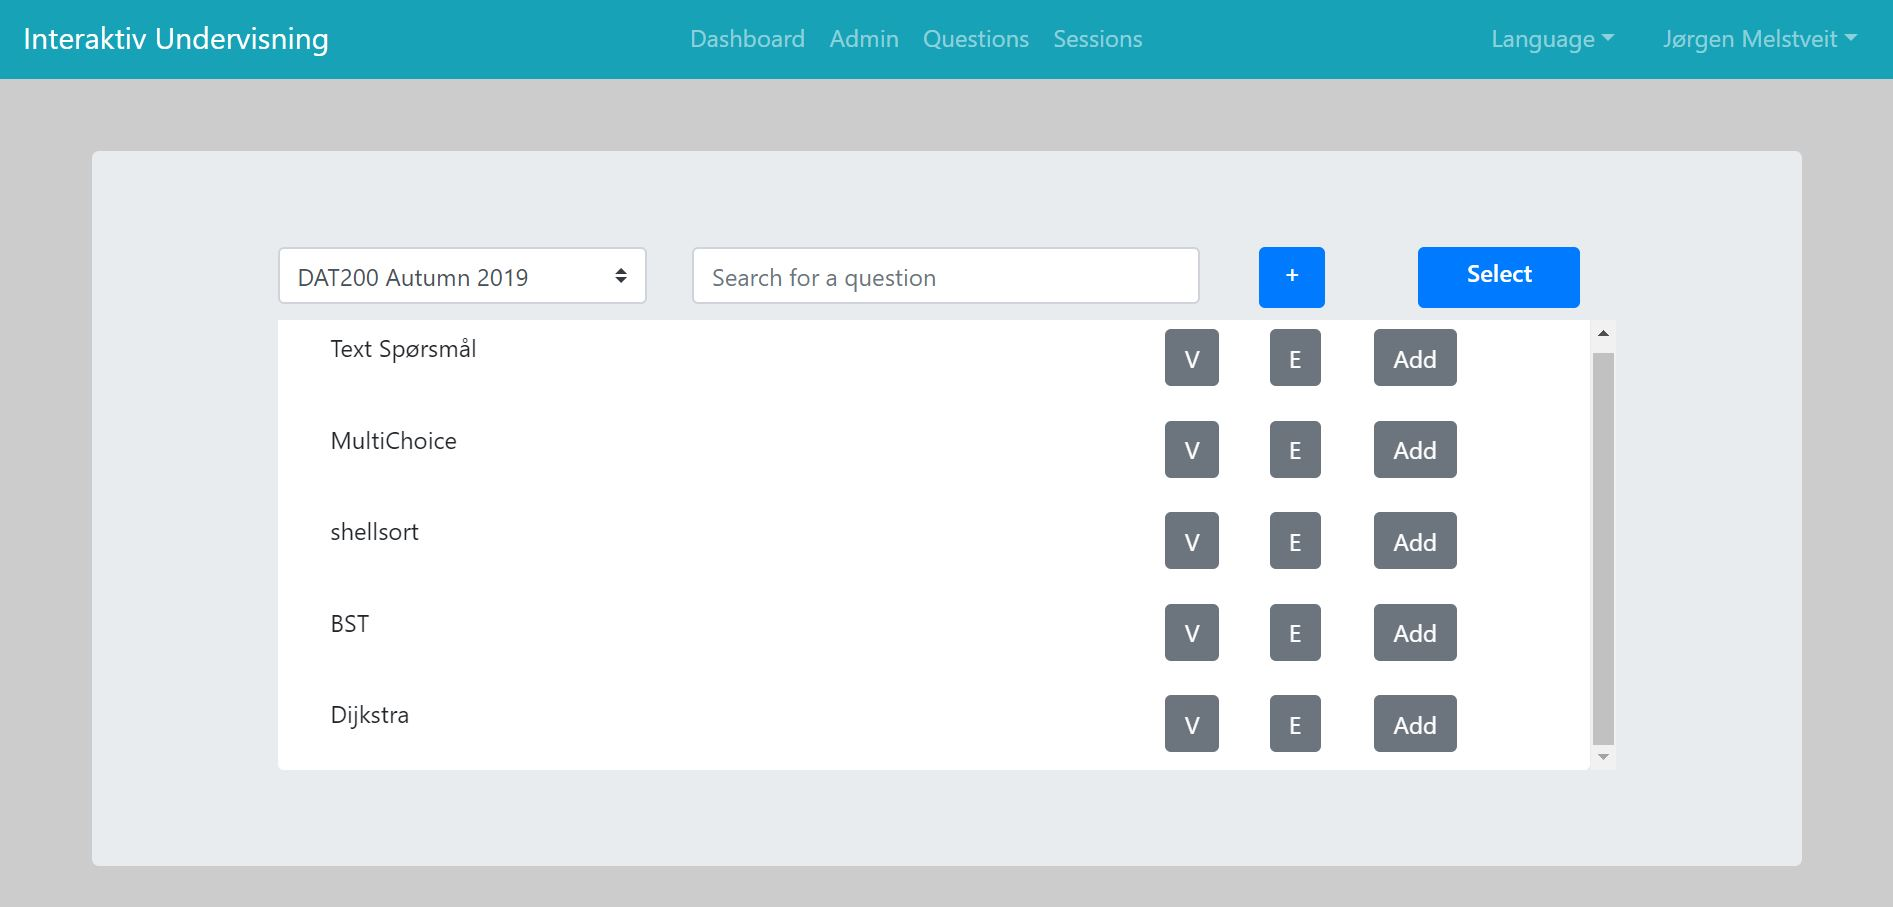
\includegraphics[width=0.80\linewidth]{/createQuestion/questionvueEnglish}
    \caption{The figure displays an image of the Questions component. It is primarily used for allowing users to create new questions for a selected course. }
    \label{fig:questionVue}
\end{figure}
\noindent
Clicking the "+" button reveals the EditQuestion component which contains a Bootstrap modal element that has all the needed forms for creating a question. EditQuestion is a component that is used for both adding new questions and editing existing questions. The main differences between the add and edit operations for the component are the following:
\begin{itemize}
\item[-] The title of the modal is different. Either it is going to be “New Question” for the add functionality or “Edit Question” for the edit functionality.
\item[-] The edit functionality needs to load the question data from the database and fill in the forms with the correct information. 
\item[-] The request sent to the server with the question information is different. The server requests are different primarily to distinguish between the insert and update SQL commands used on the database.
\end{itemize} 
Originally there were two components used for the two operations, but this was later changed in development because having two components that were practically the same was deemed unnecessary. The modal in EditQuestion is divided into three parts, namely Basic Information, Media and Solution type.  These parts can be opened and closed to the user’s preference, where basic information is open by default and the other parts are closed. The basic Information part contains an input field for assigning the question title, a text area for giving a question description, a time input field and a time slider for assigning time. The fields use v-model to mount to the object \code{newQuestion}. A v-model is a two-way connection between a variable and a HTML element. The variable has to be a property on the \code{props} or the \code{data} object. This makes sure that if the variable value is changed either by functions or by user interaction, both will have access to the updated value.  The values assigned from the different form inputs are stored in the \code{data} property of the Vue context.
The time slider and time input use different value formats, because of this, the time slider is linked with the \code{time} property. The time input uses a computed method to convert the \code{time} property to a text value. If the user changes the time input the computed method will convert it back to an integer value. This means that these elements always change their value depending on the other, resulting in them having the same value. If the time is set to “00:00”, then the question will not have a timer when used in a session. In the database, the value is stored as an integer, and if it is 0, it is stored as -1.
\\[11pt]
The media part is an optional part when making a new question. The “Media” part on the EditQuestion component consists of a select element and a part that displays added media at the bottom. The select element is used for selecting the wanted media type. If the select element has the value “images”, the media part is set up for adding images to the question. This, in turn, makes a button appear with the text “Choose a file to upload...”. This button is used for adding an image to the question. Once the button is clicked a file browser is displayed for the user and allows them to choose an image on their computer and put it into their question. If an image is chosen, the EditQuestion component takes the image and validates it. It is important to check that the file is an actual image file. If the validation passes, the image is turned into a buffer. When a question with an image is sent to the server. It will first move the image buffer into a temporary list. Then the server creates file paths for each image and places them into the question object. After the question has been stored in the database, the image buffers are turned into image files and stored in the file system. Whenever a question is obtained from the database that has images, the server loads the images by using the file paths stored in the question object. When the image is going to be used on the client, a new buffer is created based on the image and stored in the question object. A question cannot have too many images assigned to it, as this would take up a lot of the needed data. The total amount of files attached to a question cannot exceed 1.5MB, and the user will get a warning once the amount exceeds 500KB. These checks will run in the validation once an image is added to the question. Images in a question is displayed as a preview with filename, file size, and a small image on the side.
\\[11pt]
"Tables" is another media that can be added to a question. If "Tables" is selected from the media selector, a window for editing a table appears. This window contains buttons to add/remove rows and columns. Each cell contains an input field to add a value. After a table have been saved to a question, it appears as a preview at the bottom, where the user can see all the added tables and what their contents. The last media that is possible to include is a "Graphs" made with the GraphDrawer. This feature allows the user to draw with the GraphDrawer and save the canvas as an image. This image is also added to the overall image sizes. A combination of graphs and images cannot exceed 1.5MB. When running a session, a question contains tables and media that the user uploaded, drew using the GraphDrawer.
\\[11pt]
The solution type part focuses on determining the question type of the new question and for creating the question's solution. The type decides what format the question has for both the solution and for the client during a session. Most of the question types available are usually centered around a data structure or an algorithm from the DAT200 or DAT110 course. There are also other question types like multiple choice and text questions. The chosen question type alters the available options for the solution so that the user can fill in the information needed for the chosen algorithm or data structure. For instance, Binary Search Tree, AVL, Python, and Dijkstra question types all require the GraphDrawer tool. The solution for questions revolving data structures and algorithms are created on the server in the solution generator. The user only needs to give the necessary information for the question so that it is possible for the student to solve it, and for the server to be able to create the solution. The are two reasons for having the server handle the solution generation. The first reason is to keep it away from clients participating in a session. The second reason is that forcing the user to write the entire solution for every question would be rather tedious. Not to mention reducing the chances of having the solution being written incorrectly.
\begin{figure}[H]
    \centering
    \begin{subfigure}{0.70\linewidth}
        \includegraphics[width=\linewidth]{/createQuestion/editQuestionUnopenedEnglish}
        \caption{This figure displays an image of the EditQuestion component when all the three parts Basic Information, Media and Solution type are hidden. Clicking on the labels reveals the content of chosen part.}
        \label{fig:editquestionUnopened}
    \end{subfigure}
    \begin{subfigure}{0.70\linewidth}
        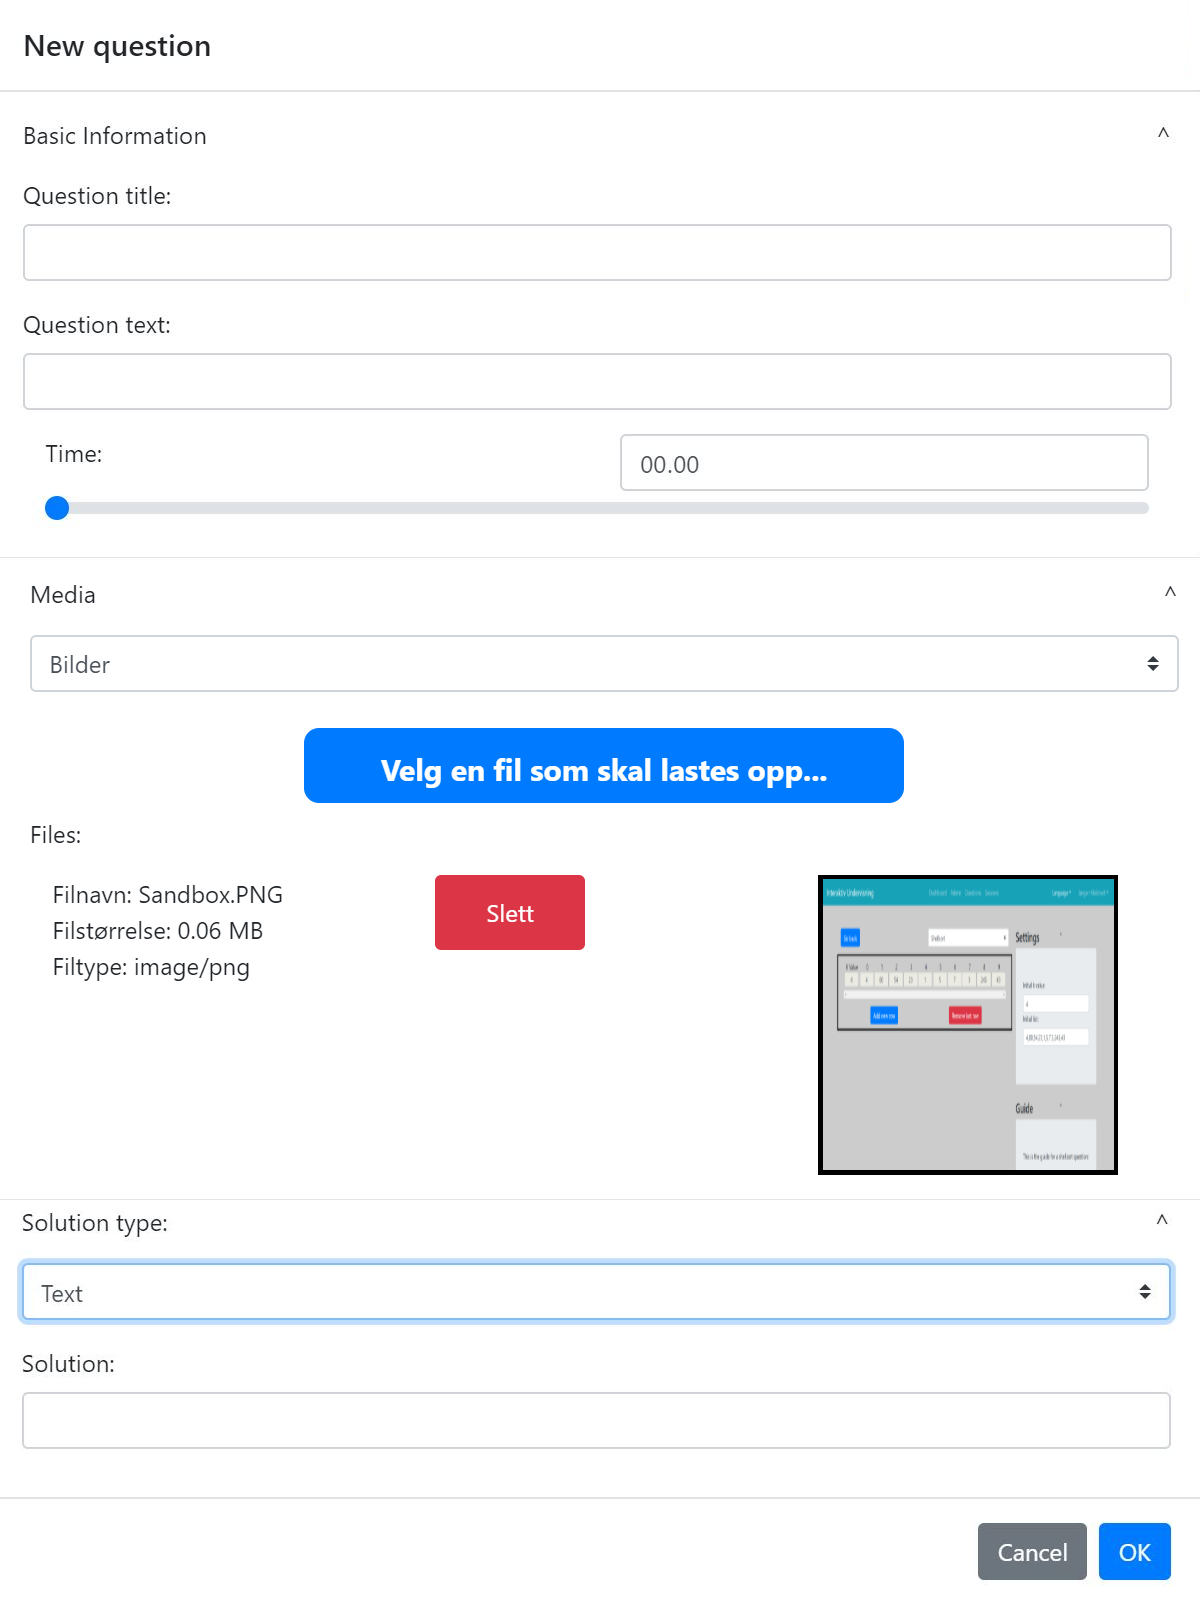
\includegraphics[width=\linewidth]{/createQuestion/editQuestionCombined}
        \caption{This figure displays an image of the EditQuestion component when all the three parts Basic Information, Media and Solution type are displayed. Clicking on the labels hides the content of the chosen part.}
        \label{fig:editquestionOpened}
    \end{subfigure}
\end{figure}
\noindent
Once the question is finished the question information is sent to the server through a socket request. The data sent to the server is the \code{newQuestion} object defined in the function \code{initializeState} in the component. Since all the properties in the \code{newQuestion} object are linked to the component, the server should have all the information it needs to generate the question solution. However, to avoid any problems regarding storing faulty questions on the server, the question information will first need to be validated by the server's validation checker. The user must at minimum fill in the information in basic information and solution type for the wanted question to be valid. The question information sent to the server is first validated on the basic information in the question. After that, if the question has an attached media to it, it is validated next. Finally, another validation test that is determined by the given question's type. All the question types have their own unique check in the validation checker which are separated in different JavaScript files. If the validation checker returns false, then the question failed the validation criteria, the errors given by the validation checker is returned to the EditQuestion component as an alert box. The errors received by the validation may vary, but all error messages that were triggered is shown. The error messages are stored in the locale files. If the validation succeeds, then the information is sent to the solution generator that generates the appropriate solution in accordance with the question's type. The solution generator has a structure similar to that of the validation checker. Each solution generator has its own JavaScript file. The main "SolutionGenerator.js" file is used to link the question to its proper solution generator function. If the question requires the GraphDrawer tool to visualize its solution, then the solution object created from the generator is going to follow a certain format. The solution object here is an array that contains all the steps necessary to solve the exercise marked with a type variable assigned with the action taken at the step. The last step is going to indicate either “finish” or “done” and is always going to be the last entry in the array. It is this object that is going to be used in the solution checker during an active session. The reason why this structure is used for solutions using the GraphDrawer, is because the GraphDrawer can show the entire process of solving the chosen exercise revolving an algorithm or a data structure. However, the GraphDrawer tool requires this format for this to work.  Once this is done, the question information and solution are inserted into the question table in the database. After the question is stored in the database, the EditQuestion component is closed, and the user is returned to the Questions component. The Questions component is then going to update its question list to accommodate for the changes done on the database.
\\[11pt]
Once a question is created and listed in the Questions component, there will be more options available for the user regarding the question. The button with the drawing symbol opens the EditQuestion component and makes it possible to edit the information previously saved for the question. Do keep in mind that the changes done to the existing question are not going to be saved unless a new request is sent to the server. This means that the new question info must also be fully validated by the validation checker, and a new solution needs to be created for the solution generator to overwrite the previous solution. If the validation fails, then the edits will not be saved in the database. It is also not possible to edit a question once it has been assigned to a session. Once a question is assigned to a session, it will have its status to change to active. This is indicated on the question on the Questions component when the edit button has a gray background. The reason for not allowing any question to be altered after it has been assigned to a session is because it would affect the saved data after a session is finished. This means that when a question has been assigned to a session, then that question is deemed completed by the application and should no longer be altered.
\\[11pt]
The button with the eye symbol causes the component ShowQuestion to become visible. This component loads all the information regarding the chosen question. The ShowQuestion consist of a Bootstrap modal that has a similar design to the EditQuestion component. It is divided into the same three parts as EditQuestion, where Media is only shown in the component if any images, tables or graphs are included in the question. In the basic information section, the user can view the basic information. In the media section, the user can view all the images, tables or graphs currently linked to the question. This includes information about the file such as name, type and the size. In the solution section, the solution to the question is displayed. The shown content depends on the solution type. Text, Multichoice and Binary tree will show the answer in plain text. Every other question type will use the GraphDrawer tool to display the solution. 
\begin{figure}[H]
    \centering
    \begin{subfigure}{0.80\linewidth}
        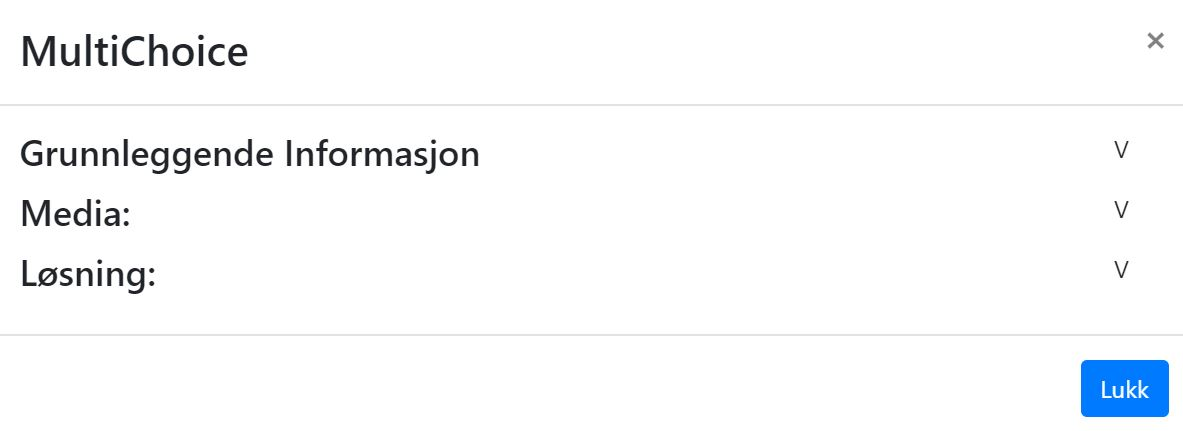
\includegraphics[width=\linewidth]{/createQuestion/showQuestionEnglishUnOpened}
        \caption{This figure displays an image of the ShowQuestion component while all the three parts are closed. Clicking on the labels  opens the chosen part.}
        \label{fig:showQuestionUnOpened}
    \end{subfigure}
    \begin{subfigure}{0.32\linewidth}
        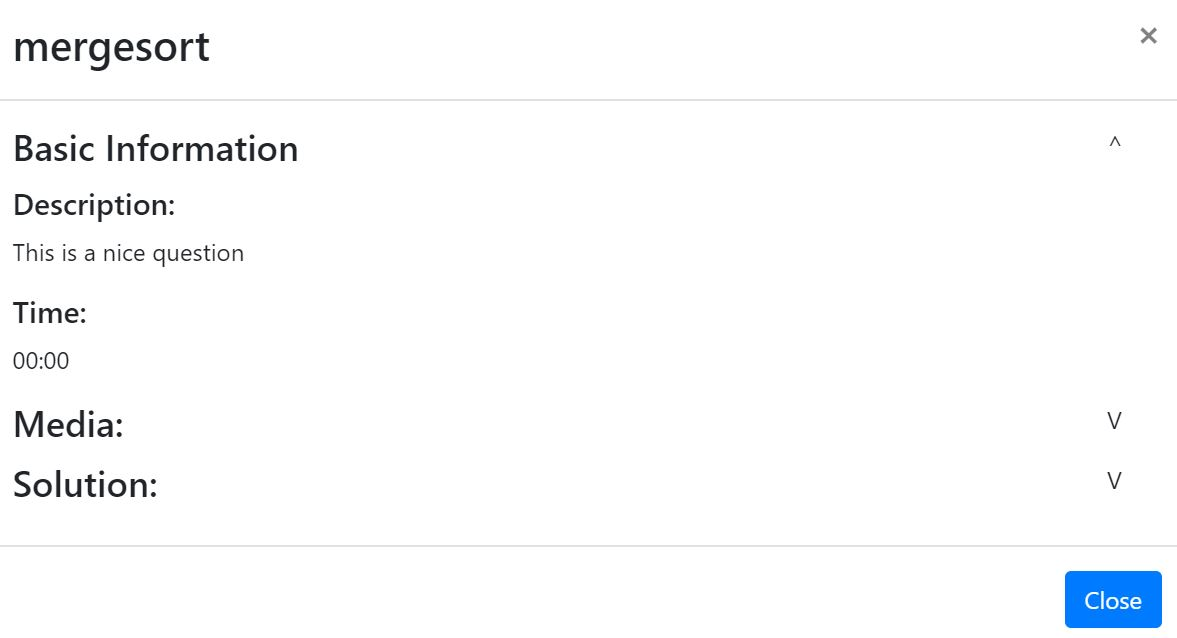
\includegraphics[width=\linewidth]{/createQuestion/showQuestionEnglishBasicOpened}
        \caption{}
        \label{fig:showQuestionBasicOpened}
    \end{subfigure}
    \begin{subfigure}{0.32\linewidth}
        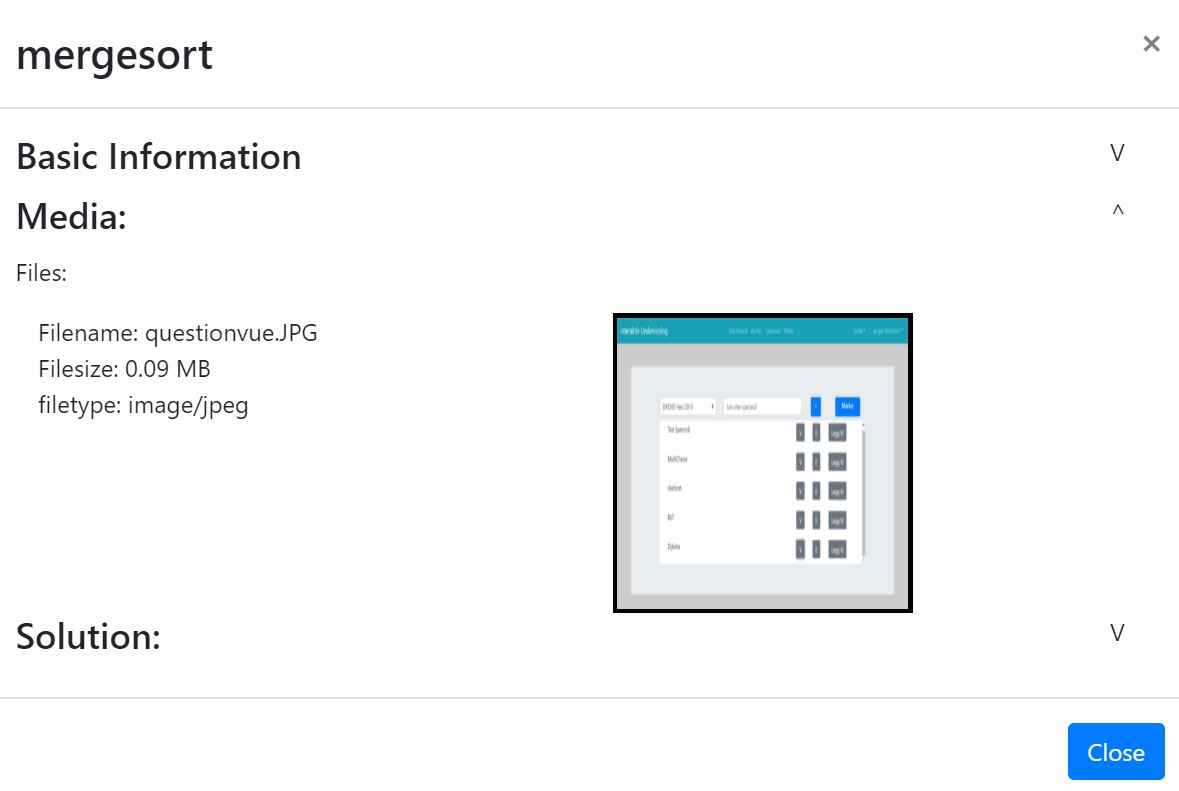
\includegraphics[width=\linewidth]{/createQuestion/showQuestionEnglishMediaOpened}
        \caption{}
        \label{fig:showQuestionMediaOpened}
    \end{subfigure}
    \begin{subfigure}{0.32\linewidth}
        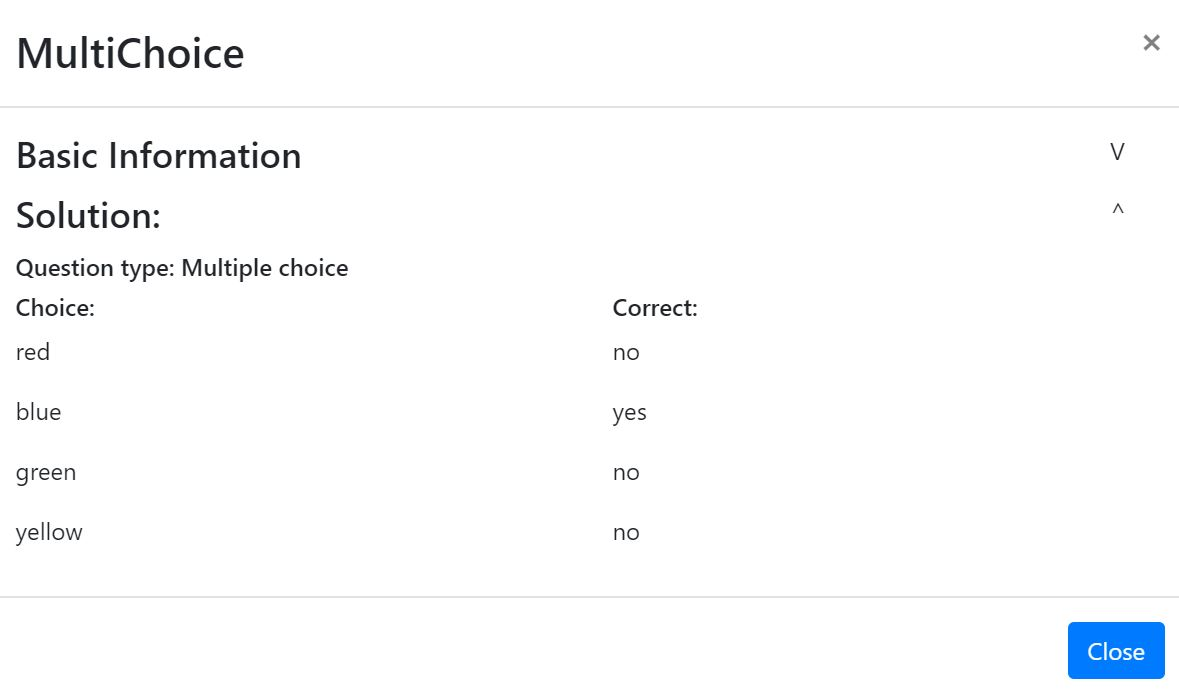
\includegraphics[width=\linewidth]{/createQuestion/showQuestionEnglishSolutionOpened}
        \caption{}
        \label{fig:showQuestionSolutionOpened}
    \end{subfigure}
\end{figure}
\noindent
The last button labeled Add will open the AddQuestionToSession component. This component displays a select element containing all currently available sessions in the database. The user can select one of the sessions and add the chosen question to the chosen session. This was implemented to give admins the option of adding more questions to an existing session.
\\[11pt]
Lastly, the Questions component makes it possible to mark questions in the list by clicking on the button with the label “Select”. Once the button is clicked, the user has the option of either copying the selected questions to another course or deleting the questions from the current course. When a question is copied an identical question is created where the course id foreign key is assigned to the chosen course. The copy is stored in the database. When a question is deleted, the question is simply removed from the database. To exit the select mode click on the select button again, which now has the label “Close”. The copy button opens the CopyQuestions component, while the delete button opens the DeleteQuestions component. If the user attempts to copy or remove without having selected a question, then an alert box appears stating that there are no questions currently selected. Keep in mind that it is not possible to remove questions from a course if it has already been used in a session. The reason for this is that the question information is still needed for Feide users to look at their previous participated sessions. If the question were to be removed after having been used in a session, then the student would not have access to the question information. Therefore, the students would have no way of looking at their old session results. 
\\[11pt]
The question structure for this application was specifically chosen such that it would be easier for developers to implement and add new questions types. Excluding the work that is needed for writing the actual data structure or algorithm and its solution format. All that is required in order to add a new question type to a session is the following:
\begin{enumerate}
	\item Create a Vue component in both the questionResultScreenAnswer and questionResultScreenSolution directories. These are used for the DisplayQuestion component. The DisplayQuestion component is used for showing question results for each question.
	\item Add a b-form-group element to the EditQuestion component where only the necessary form items or Graphdrawer properties are set so that the user can create the new question type.
	\item If the question type requires certain unique information, then an extra property in the \code{newQuestion.objects} in the \code{initializeState} function should also be assigned and modeled appropriately to the HTML element in the form group.
	\item Add a JavaScript file in the validation checker for stopping illegal actions to the new type. 
	\item Implement the solution generator for the question type which is going to create the format for the solution object stored in the database.
	\item Add the new question type to question type array in the database.js file.
	\item Finally, implement a solution checker that is going to verify that the student answered the question correctly according to the solution object. 
	\item Add text to the locale files if the new question type requires them.
\end{enumerate}
